%************************************************
\chapter{Efficient Evaluation}\label{ch:efficient_eval}
%************************************************

In this chapter, we derive an equivalent metric first with the standard two-way SED using only intersecting 
dimensions to significantly reduce its cost, and secondly, generalising to the multi-way MSED whereby if there are $n$ input vectors we only need to consider dimensions that are non-zero in $> 1$ of the input vectors, avoiding the cost of calculating logs.  

We evaluate over both sparse vectors and inverted indices which allow parallel evaluation over large data spaces.  We show that a lower bound can be efficiently maintained during calculation so that the calculation may be eagerly abandoned.
\section{Avoiding calculation of the mean}
We consider the efficient evaluation of JSD, since it can be used in the calculation of MSED.  In particular, we are interested in an incremental evaluation since evaluation over large collections can be achieved through the use of an inverted index data structure, saving space.
\subsection{2-way case}
Although it appears that JSD requires the construction of a new vector $\mathbf{z}$, in fact, $\mathbf{z}$ does not need to be constructed.  Working with the vector notation from section \ref{vector_space} we can see this as follows
\begin{align}
    JSD(\mathbf{x}, \mathbf{y}) &= H_b(\mathbf{z}) - \frac{1}{2}(H_b(\mathbf{x}) + H_b(\mathbf{y}))\\
    &= -\sum_i z_i \log_b z_i - \frac{1}{2}(-\sum_i  x_i \log_b x_i - \sum_i  y_i \log_b y_i)\\
    &= -\frac{1}{2}\sum_i 2 \cdot z_i \log_b z_i - (x_i \log_b x_i + y_i \log_b y_i)\\
    &= \frac{1}{2}\sum_i  x_i \log_b x_i + y_i \log_b y_i  - (x_i+y_i) \log_b \frac{(x_i+y_i)}{2}
\end{align}  
%
avoiding the construction of $\mathbf{z}$.

Using base 2 logs allows the elimination of yet more terms:
%
\begin{align}
JSD(\mathbf{x}, \mathbf{y}) &= \frac{1}{2}\sum_i  x_i \log_2 x_i + y_i \log_2 y_i - (x_i+y_i)(\log_2 (x_i+y_i) - 1)\\
 &= \frac{1}{2}\sum_i  x_i \log_2 y_i  + x_i \log_2 y_i - (x_i+y_i) \log_2 (x_i+y_i) + x_i+y_i
\intertext{and, since $\sum_i x_i = \sum_i y_i=1$,}
JSD(\mathbf{x}, \mathbf{y}) &= 1 + \frac{1}{2}\sum_i  x_i \log_2 x_i + y_i \log_2 y_i - (x_i+y_i) \log_2 (x_i+y_i)
\intertext{Since we are interested in the incremental evaluation, we negate the summand function and name it:}
\F(x,y) &= (x+y) \log_2 (x+y) - x \log_2 x  - y \log_2 y
\intertext{giving:}
JSD(\mathbf{x}, \mathbf{y}) &= 1 - \frac{1}{2}\sum_i  \F(x_i,y_i)
\end{align}
where if either (or both) of $x_i$ or $y_i$ is equal to zero then so is $\F(x_i,y_i)$, thus only the non-zero intersection is required; that is, $\F(x_i,y_i)$ need only be evaluated when $x_i \neq 0$ and $y_i \neq 0$. 
%Evaluation over large collections can be achieved through the use of an inverted index data structure, saving space as well.
\begin{figure}
  \centering
  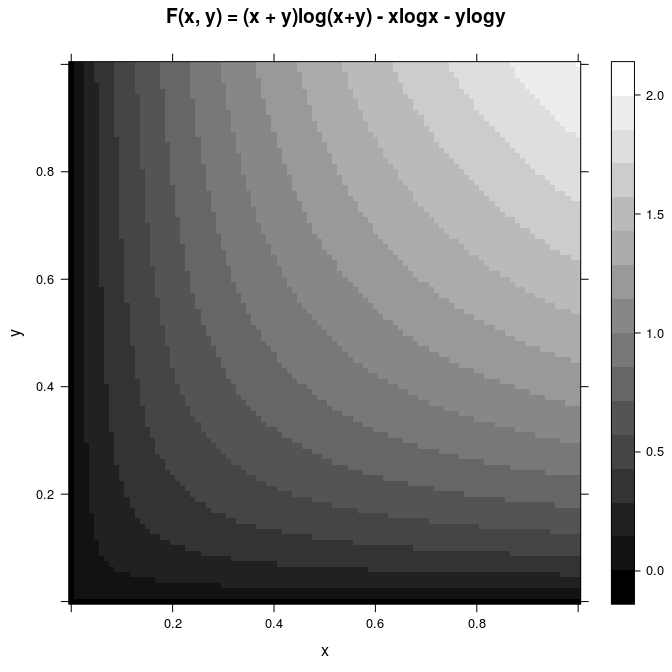
\includegraphics[width=4in]{gfx/F(x,y)}
  \caption[The function $\F$ on all possible inputs]
   {The function $\F$ on all possible inputs}
   \label{fig:F}
\end{figure}

\subsection{multi-way case}
In the multi-way case we follow the same reasoning.  Starting with the definition of $JSD$ we avoid the construction of $\mathbf{z}$ as follows:
%Although it appears that JSD requires the construction of a new vector $\mathbf{z}$, in fact, $\mathbf{z}$ does not need to be constructed.  Working with the vector notation from section \ref{vector_space} we can see this as follows
\begin{align}
    JSD(\mathbf{x}^{(1)}, \ldots, \mathbf{x}^{(n)}) &= H_b(\mathbf{z}) - \frac{1}{n}(\sum_j H_b(\mathbf{x}^{(j)}))\\
    &= -\sum_i z_i \log_b z_i - \frac{1}{n}(\sum_j -\sum_i  x^{(j)}_i \log_b x^{(j)}_i)\\
    &= -\frac{1}{n}\sum_i n \cdot z_i \log_b z_i - (\sum_j x^{(j)}_i \log_b x^{(j)}_i )\\
    &= \frac{1}{n}\sum_i  (\sum_j x^{(j)}_i \log_b x^{(j)}_i )  - (\sum_j x^{(j)}_i) \log_b \frac{(\sum_j x^{(j)}_i)}{n}
\end{align}  
%

This time using base $n$ logs allows the elimination of extra terms:
%
\begin{align}
JSD(\mathbf{x}^{(1)}, \ldots, \mathbf{x}^{(n)}) &= \frac{1}{n}\sum_i   (\sum_j x^{(j)}_i \log_n x^{(j)}_i ) - (\sum_j x^{(j)}_i) (\log_n \sum_j x^{(j)}_i - 1)\\
 &= \frac{1}{n}\sum_i (\sum_j x^{(j)}_i \log_n x^{(j)}_i ) - (\sum_j x^{(j)}_i) \log_n (\sum_j x^{(j)}_i) + (\sum_j x^{(j)}_i)
\intertext{and, since $\sum_i x^{(j)}_i = \sum_i x^{(k)}_i=1$, for any j, k}
JSD(\mathbf{x}^{(1)}, \ldots, \mathbf{x}^{(n)}) &= 1 + \frac{1}{n}\sum_i  (\sum_j x^{(j)}_i \log_n x^{(j)}_i ) -  (\sum_j x^{(j)}_i) \log_n (\sum_j x^{(j)}_i)
\intertext{again, we are interested in the incremental evaluation, so we generalise the $\F$ function from the 2-way case:}
\F(x^{(1)}, \ldots, x^{(n)}) &= (\sum_j x^{(j)}) \log_n (\sum_j x^{(j)}) - (\sum_j x^{(j)} \log_n x^{(j)})
\intertext{giving:}
JSD(\mathbf{x}^{(1)}, \ldots, \mathbf{x}^{(n)}) &= 1 - \frac{1}{n}\sum_i  \F(x^{(1)}_i,\ldots,x^{(n)}_i)
\end{align}
As before, we notice that $\F$ is equal to zero when $n - 1$ or more of the $n$ input values is zero.  Thus, we can avoid the expensive calculation of the logs and replace it with the cheaper count of zeros.
\section{Early termination}
%
The outcome of the metric, with range queries in similarity search, is of no interest if it is greater than the threshold $r$. We now show a way of optimising the calculation further.

The threshold requirement is written
\begin{align}
&&            &\frac{n^{1 - \frac{1}{n}\sum_{i = 1}^n  \F(x^{(1)}_i,\ldots, x^{(n)}_i)} - 1}{n - 1}   & \leq & & &r\\
&\Rightarrow& &n^{1 - \frac{1}{n}\sum_{i = 1}^n  \F(x^{(1)}_i,\ldots, x^{(n)}_i)} - 1   & \leq & & &(n - 1)r\\
&\Rightarrow& &1 - \frac{1}{n} \sum_{i = 1}^n  \F(x^{(1)}_i,\ldots, x^{(n)}_i)          & \leq & & &\log_n((n - 1)r + 1)\\
&\Rightarrow& &- \frac{1}{n} \sum_{i = 1}^n  \F(x^{(1)}_i,\ldots, x^{(n)}_i)          & \leq & & &\log_n((n - 1)r + 1) - 1\\	
&\Rightarrow& &\sum_{i = 1}^n  \F(x^{(1)}_i,\ldots, x^{(n)}_i)                          & \geq & & &n -  n\log_n((n - 1)r + 1)	
\end{align}
$\F$ can be seen as a similarity accumulator, and the term $n\log_n((n - 1)r + 1)$ as the maximum shortfall that may occur in order for the threshold $r$ not to be exceeded. 

If, at any point of the iterative calculation, we can determine that it is impossible for the value of $\sum_{i = 1}^n  \F(x^{(i)},\ldots, x^{(n)})$ to reach the threshold of $n -  n\log_n((n - 1)r + 1)$, then the calculation may be abandoned.

\begin{figure}
  \centering
  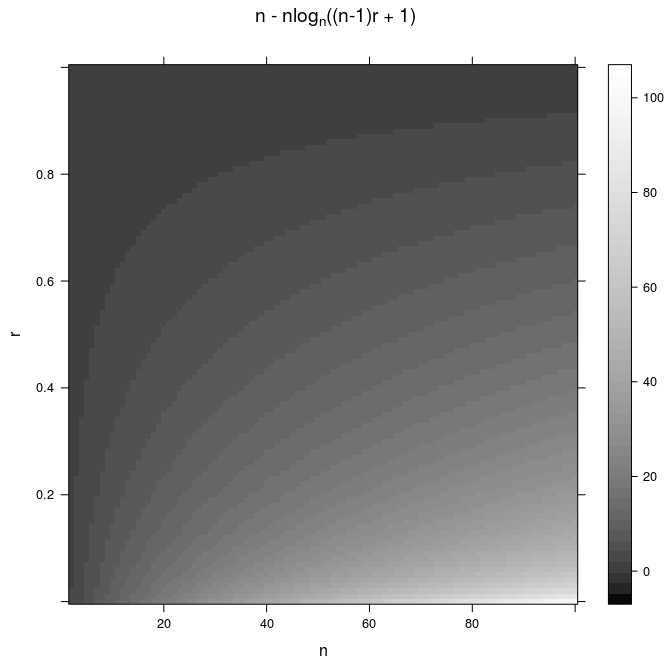
\includegraphics[width=4in]{gfx/threshold}
  \caption[Similarity lower bounds]
   {Similarity lower bounds}
   \label{fig:threshold}
\end{figure}

We calculate an upper bound for $\sum_{i = 1}^n  \F(x^{(i)},\ldots, x^{(n)})$ after $k$ stages of the iteration by consideration of the sum of terms:
\begin{equation}
\sum_{i = 1}^n  \F(x^{(i)},\ldots, x^{(n)}) = \sum_{i = 1}^k  \F(x^{(i)},\ldots, x^{(n)}) + \sum_{i = k+1}^n  \F(x^{(i)},\ldots, x^{(n)})
\end{equation}
At stage $k$, the value of the left hand term is known, and using the Jensen inequality we can calculate an upper bound for the right-hand term:
\begin{align}\label{equation_threshold}
&& &\sum_{i=k+1}^n  \F(x^{(i)},\ldots, x^{(n)}) & \le & &  &\F\left(\sum_{i=k+1}^n x^{(1)}_i,\ldots,\sum_{i=k+1}^n x^{(n)}_i\right)\\
&\Rightarrow& &\sum_{i=k+1}^n  \F(x^{(i)},\ldots, x^{(n)}) & \le & & &\F\left(1 - \sum_{i=1}^k x^{(1)}_i,\ldots, 1 - \sum_{i=1}^k x^{(n)}_i \right)
\end{align}
without knowledge of even the number of dimensions still to be computed.

Thus if at any stage $k$ the inequality
\begin{equation}
\sum_{i = 1}^k  \F(x^{(i)},\ldots, x^{(n)}) + \F\left(1 - \sum_{i=1}^k x^{(1)}_i,\ldots, 1 - \sum_{i=1}^k x^{(n)}_i \right) < n -  n\log_n((n - 1)r + 1)
\end{equation}
becomes true the calculation may be terminated early with the knowledge that the distance falls out with the range of the query.

Whether the optimisation based on this observation is worth applying or not depends entirely on the context of the calculation; it requires the calculation of an extra application of $\F$ and, if applied at each stage of the calculation, would only be cost-effective if a saving equivalent to half the number of stages was achieved. This is not to say that the observation is of no use, and in particular there may be circumstances where an I/O saving can be achieved.

%--------------------------------------------------------------------------------------------------%	
\section{Evaluation}
\label{section_evaluation}
Based on the above algebraic observations, we implemented five different methods of evaluating the metric, as follows.  All of which avoided the calculation of the mean vector:

\begin{singlespace*} 
\begin{description}\item[Inverted Index] Using an inverted index (skipping dimensions where > n-1 values are 0);
\item[Inverted Index ET] using an inverted index with early termination (skipping dimensions where > n-1 values are 0).
\item[Sparse Vectors] All dimensions of the vectors being compared are accessed;
\item[Sparse Vectors 2] skipping dimensions where > n-1 values are 0;
\item[Sparse Vectors 3] skipping dimensions where > n-1 values are 0, with early termination;
\end{description}
\end{singlespace*}
\begin{figure}[h!]
\centering
\subfloat[Simple Vector Representation] 
{\label{fig:simple_vector_representation}
%%
% Dense vectors
%%
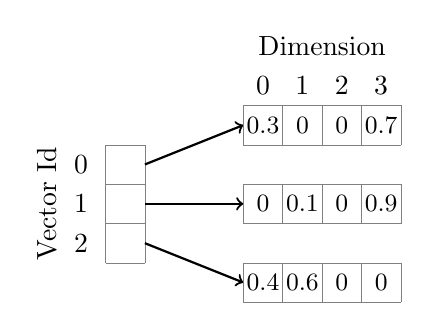
\begin{tikzpicture}
\node[rotate=90] at (-0.75, 1.5) {Vector Id};
\node [left] at (-0.1, 2) {0};
\node [left] at (-0.1, 1.5) {1};
\node [left] at (-0.1, 1) {2};

\node at (2.75, 3.5){Dimension};
\node at (2, 3) {0};
\node at (2.5, 3) {1};
\node at (3, 3) {2};
\node at (3.5, 3) {3};

\draw [help lines, step=0.5,xshift=0cm,yshift=0.75cm] (0,0) grid (0.5,1.5);
\draw[thick,->] (0.5,1) -- (1.75,0.5);
\draw[thick,->] (0.5,1.5) -- (1.75,1.5);
\draw[thick,->] (0.5,2) -- (1.75,2.5);

\draw [help lines, step=0.5,xshift=-0.25cm,yshift=0.25cm] (2 - 0.002, 2 - 0.002) grid +(2.002,0.5+0.002);
\foreach \x/\y/\z in {2/2.5/0.3, 2.5/2.5/0, 3/2.5/0, 3.5/2.5/0.7}
	\node[font=\small] at (\x, \y) {\z};

\draw [help lines, step=0.5,xshift=-0.25cm,yshift=-0.75cm] (2 - 0.002, 2 - 0.002) grid +(2.002,0.5+0.002);
\foreach \x/\y/\z in {2/1.5/0, 2.5/1.5/0.1, 3/1.5/0, 3.5/1.5/0.9}
	\node[font=\small] at (\x, \y) {\z};
	
\draw [help lines, step=0.5,xshift=-0.25cm,yshift=-1.75cm] (2 - 0.002, 2 - 0.002) grid +(2.002,0.5+0.002);
\foreach \x/\y/\z in {2/0.5/0.4, 2.5/0.5/0.6, 3/0.5/0, 3.5/0.5/0}
	\node[font=\small] at (\x, \y) {\z};
\end{tikzpicture}
} \quad
\subfloat[Sparse Vector Representation] 
{\label{fig:sparse_vector_representation}
%%
% Sparse vectors
%%
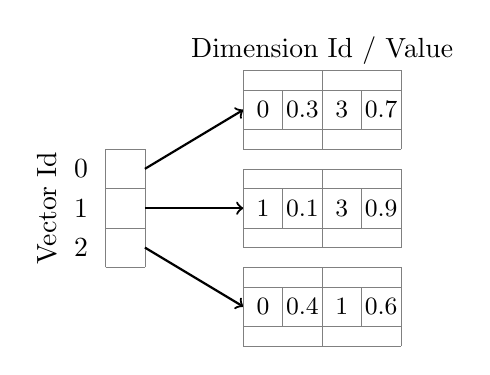
\begin{tikzpicture}
\node[rotate=90] at (-0.75, 1.5) {Vector Id};
\node [left] at (-0.1, 2) {0};
\node [left] at (-0.1, 1.5) {1};
\node [left] at (-0.1, 1) {2};

\node at (2.75, 3.5){Dimension Id / Value};

\draw [help lines, step=0.5,xshift=0cm,yshift=0.75cm] (0,0) grid (0.5,1.5);
\draw[thick,->] (0.5,1) -- (1.75,0.25);
\draw[thick,->] (0.5,1.5) -- (1.75,1.5);
\draw[thick,->] (0.5,2) -- (1.75,2.75);

\draw [help lines, step=1,xshift=-0.25cm,yshift=0.25cm] (2 - 0.002, 2 - 0.002) grid +(2.002,1+0.002);
\draw [help lines, step=0.5,xshift=-0.25cm,yshift=0.5cm] (2 - 0.002, 2 - 0.002) grid +(2.002,0.5+0.002);
\foreach \x/\y/\z in {2/2.75/0, 2.5/2.75/0.3, 3/2.75/3, 3.5/2.75/0.7}
	\node[font=\small] at (\x, \y) {\z};

\draw [help lines, step=1,xshift=-0.25cm,yshift=-1cm] (2 - 0.002, 2 - 0.002) grid +(2.002,1+0.002);
\draw [help lines, step=0.5,xshift=-0.25cm,yshift=-0.75cm] (2 - 0.002, 2 - 0.002) grid +(2.002,0.5+0.002);
\foreach \x/\y/\z in {2/1.5/1, 2.5/1.5/0.1, 3/1.5/3, 3.5/1.5/0.9}
	\node[font=\small] at (\x, \y) {\z};
	
\draw [help lines, step=1,xshift=-0.25cm,yshift=-2.25cm] (2 - 0.002, 2 - 0.002) grid +(2.002,1+0.002);
\draw [help lines, step=0.5,xshift=-0.25cm,yshift=-2cm] (2 - 0.002, 2 - 0.002) grid +(2.002,0.5+0.002);
\foreach \x/\y/\z in {2/0.25/0, 2.5/0.25/0.4, 3/0.25/1, 3.5/0.25/0.6}
	\node[font=\small] at (\x, \y) {\z};
\end{tikzpicture}
} \quad
\subfloat[Inverted Index Representation] 
{\label{fig:inverted_index_representation}

%%
% Inverted Index
%%
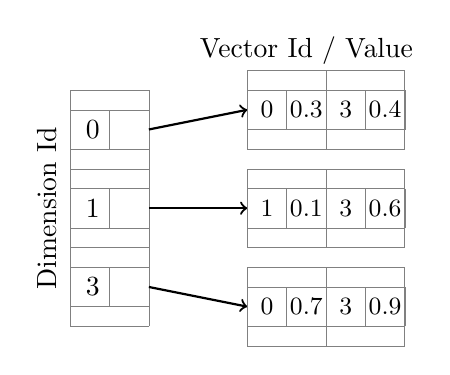
\begin{tikzpicture}
\node[rotate=90] at (-0.3, 1.5) {Dimension Id};
\node [left] at (0.5, 2.5) {0};
\node [left] at (0.5, 1.5) {1};
\node [left] at (0.5, 0.5) {3};

\node at (3, 3.5){Vector Id / Value};

\draw [help lines, step=1,xshift=0cm,yshift=0cm] (0,0) grid (1,3);
\draw [help lines, step=0.5,xshift=0cm,yshift=0.25cm] (0,0) grid (1,0.5);
\draw [help lines, step=0.5,xshift=0cm,yshift=1.25cm] (0,0) grid (1,0.5);
\draw [help lines, step=0.5,xshift=0cm,yshift=2.25cm] (0,0) grid (1,0.5);
\draw[thick,->] (1,0.5) -- (2.25,0.25);
\draw[thick,->] (1,1.5) -- (2.25,1.5);
\draw[thick,->] (1,2.5) -- (2.25,2.75);

\draw [help lines, step=1,xshift=0.25cm,yshift=0.25cm] (2 - 0.002, 2 - 0.002) grid +(2.002,1+0.002);
\draw [help lines, step=0.5,xshift=0.25cm,yshift=0.5cm] (2 - 0.002, 2 - 0.002) grid +(2.002,0.5+0.002);
\foreach \x/\y/\z in {2/2.75/0, 2.5/2.75/0.3, 3/2.75/3, 3.5/2.75/0.4}
	\node[font=\small,xshift=0.5cm] at (\x, \y) {\z};

\draw [help lines, step=1,xshift=0.25cm,yshift=-1cm] (2 - 0.002, 2 - 0.002) grid +(2.002,1+0.002);
\draw [help lines, step=0.5,xshift=0.25cm,yshift=-0.75cm] (2 - 0.002, 2 - 0.002) grid +(2.002,0.5+0.002);
\foreach \x/\y/\z in {2/1.5/1, 2.5/1.5/0.1, 3/1.5/3, 3.5/1.5/0.6}
	\node[font=\small,xshift=0.5cm] at (\x, \y) {\z};
	
\draw [help lines, step=1,xshift=0.25cm,yshift=-2.25cm] (2 - 0.002, 2 - 0.002) grid +(2.002,1+0.002);
\draw [help lines, step=0.5,xshift=0.25cm,yshift=-2cm] (2 - 0.002, 2 - 0.002) grid +(2.002,0.5+0.002);
\foreach \x/\y/\z in {2/0.25/0, 2.5/0.25/0.7, 3/0.25/3, 3.5/0.25/0.9}
	\node[font=\small,xshift=0.5cm] at (\x, \y) {\z};
\end{tikzpicture}
}
\caption[]{}
\end{figure}
A number of generated spaces were used to test the mechanisms.  The generator was set to populate sparse spaces of 50, 100, 200, 400, 800, 1600 and 3200 dimensions: 50 dimensions being populated in each.  We used two types of generator, which produced what we call either shuffled or unshuffled vectors.  In the unshuffled vectors, the generator populated the first 50 dimensions of each vector; in the shuffled vectors, the generator evenly distributed the populated dimensions among the $n$ dimensions by randomly shuffling the unshuffled vectors' dimensions. Search thresholds to return $10^{-4}$ of the data were then calculated for each space.
%For 50 dense dimensions, IDIM: x, with median distance of x. 
%\begin{figure}[h]
%\centering
%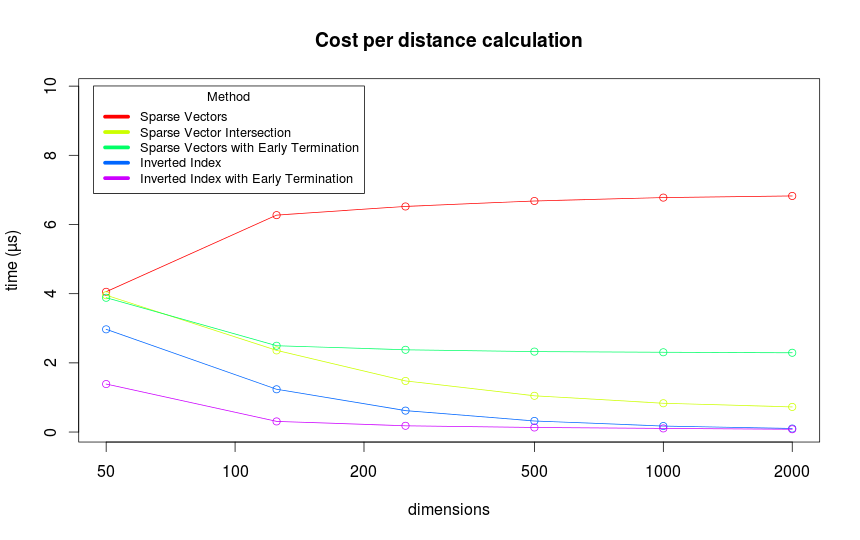
\includegraphics[width=0.9\columnwidth]{gfx/speedup_sed}
%\caption[Efficiency techniques]{distance times showing how the different techniques perform on increasingly sparse vectors}
%\label{fig:speedup_sed}
%\end{figure}

A metric index structure achieves no significant cost saving in these spaces; the space with 50 dense dimensions has an IDIM of x, with median distance of x.  IDIM increases, furthermore, with both the number of dimensions in the space and the relative sparsity.

Figure \ref{fig:sed_timings_shuffled} shows the effect of increasing the sparsity on shuffled vectors.  Initially, the sparse vectors are much quicker than the inverted index, but as the sparsity increases the inverted index becomes more efficient than the sparse vectors; this gap narrows, however, as the tuple size increases.  In all cases, the cost of maintaining the threshold invariant outweighs the saving from early termination.

\begin{figure}
        \centering
        \subfloat[2-tuple]{
				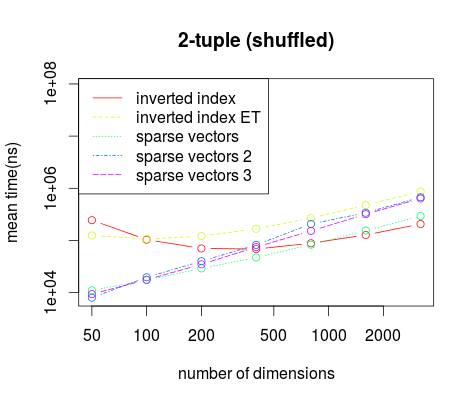
\includegraphics[width=0.35\textwidth]{gfx/times/shuffled/02.png}
                \label{fig:shuffled_02}
        }%
        ~ 
        \subfloat[4-tuple]{
				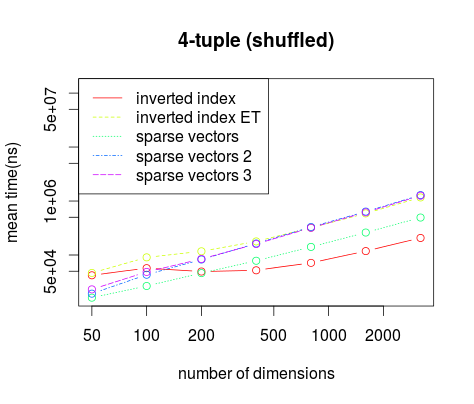
\includegraphics[width=0.35\textwidth]{gfx/times/shuffled/04.png}
                \label{fig:shuffled_04}
        }
        
         
        \subfloat[8-tuple]{
				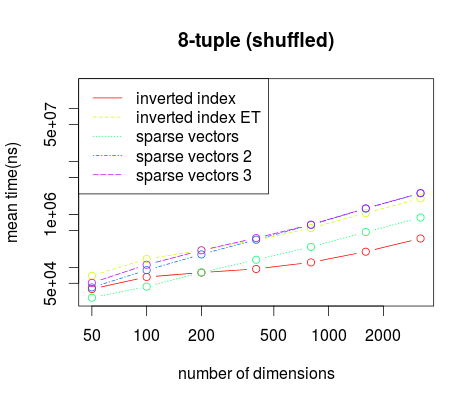
\includegraphics[width=0.35\textwidth]{gfx/times/shuffled/08.png}
                \label{fig:shuffled_08}
        }
        ~ 
        \subfloat[16-tuple]{
				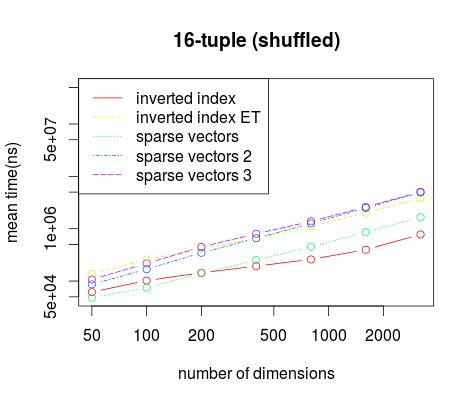
\includegraphics[width=0.35\textwidth]{gfx/times/shuffled/16.png}
                \label{fig:shuffled_16}
        }
    
        \caption[Comparison of evaluation techniques on the shuffled dataset over increasing sparsity]{Comparison of evaluation techniques on the shuffled datasets over increasing sparsity}\label{fig:sed_timings_shuffled}
\end{figure}

Figure \ref{fig:sed_timings_unshuffled} shows the effect of increasing the sparsity on unshuffled vectors.  With the 2-tuples shown in \ref{fig:unshuffled_02}, an inverted index is slower than the sparse vector representations, but benefits from using early termination.  The sparse vectors, also however, benefit significantly both from skipping dimensions and early termination.  As the tuple size is increased, the difference between sparse vectors and the inverted index narrows, and the inverted index even runs more efficiently beyond a certain point of sparsity.  Again, the higher tuple size show an impressive saving from early termination both in the inverted index and sparse vectors.   
\begin{figure}
        \centering
        \subfloat[2-tuple]{
				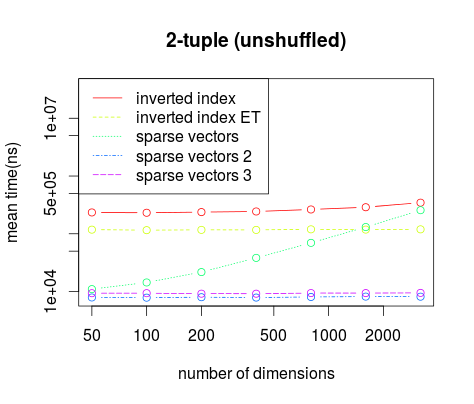
\includegraphics[width=0.35\textwidth]{gfx/times/unshuffled/02.png}
                \label{fig:unshuffled_02}
        }%
        ~ 
        \subfloat[4-tuple]{
				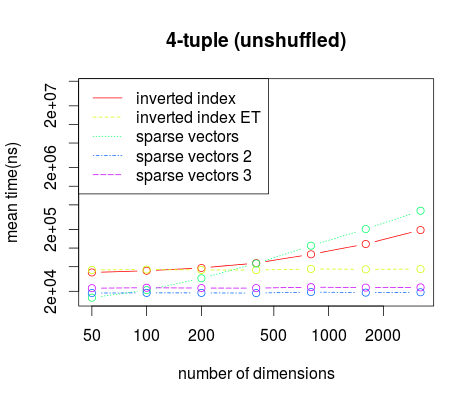
\includegraphics[width=0.35\textwidth]{gfx/times/unshuffled/04.png}
                \label{fig:unshuffled_04}
        }
        
         
        \subfloat[8-tuple]{
				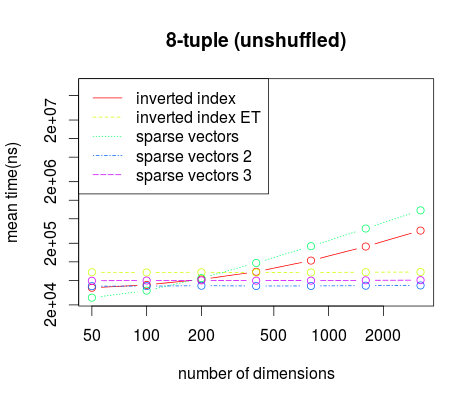
\includegraphics[width=0.35\textwidth]{gfx/times/unshuffled/08.png}
                \label{fig:unshuffled_08}
        }
        ~ 
        \subfloat[16-tuple]{
				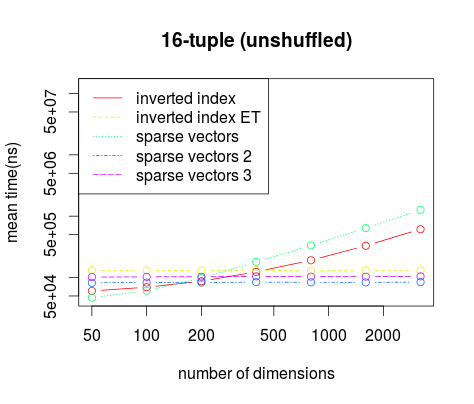
\includegraphics[width=0.35\textwidth]{gfx/times/unshuffled/16.png}
                \label{fig:unshuffled_16}
        }
    
        \caption[Comparison of evaluation techniques on the unshuffled dataset over increasing sparsity]{Comparison of evaluation techniques on the unshuffled datasets over increasing sparsity}\label{fig:sed_timings_unshuffled}
\end{figure}
% ------------------------------------------------------------------------------------------------------------------

Figure \ref{fig:sed_timings_techniques_shuffled} shows the growth of each mechanism on the shuffled data.  The growth of pattern is the same for all mechanisms: dense spaces show no extra cost when increasing the tuple size, but as the sparsity increases so does the rate of growth.
\begin{figure}
        \centering
        \subfloat[Inverted Index]{
				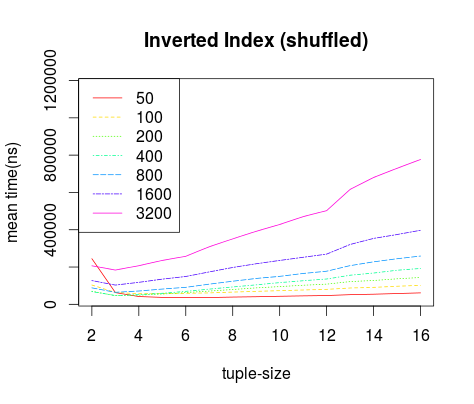
\includegraphics[width=0.35\textwidth]{gfx/times/shuffled/inverted_index.png}
                \label{fig:shuffled_inverted_index}
        }%
        ~ 
        \subfloat[Inverted Index ET]{
				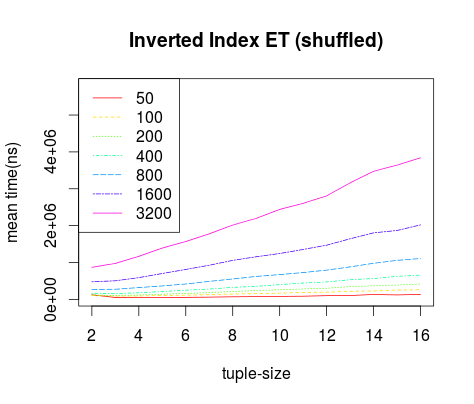
\includegraphics[width=0.35\textwidth]{gfx/times/shuffled/inverted_index_et.png}
                \label{fig:shuffled_inverted_index_et}
        }
        
         
        \subfloat[Sparse Vectors]{
				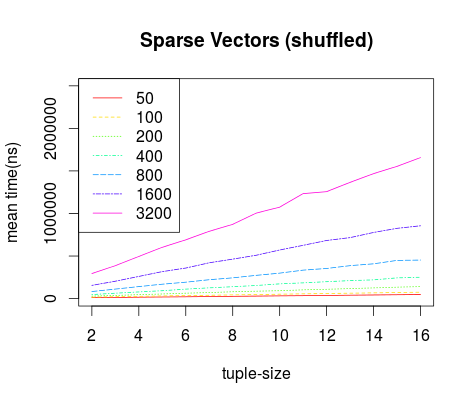
\includegraphics[width=0.35\textwidth]{gfx/times/shuffled/sparse_vectors.png}
                \label{fig:shuffled_sparse_vectors}
        }
        ~ 
        \subfloat[Sparse Vectors 2]{
				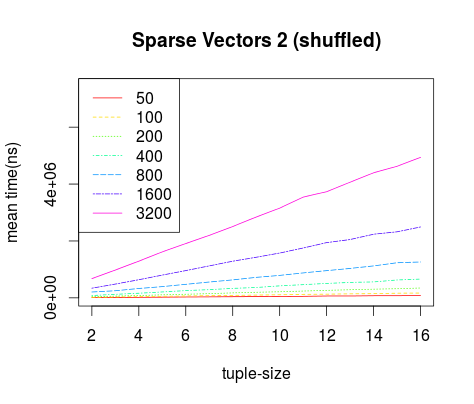
\includegraphics[width=0.35\textwidth]{gfx/times/shuffled/sparse_vectors_2.png}
                \label{fig:shuffled_sparse_vectors_2}
        }
        
        
        \subfloat[Sparse Vectors 3]{
				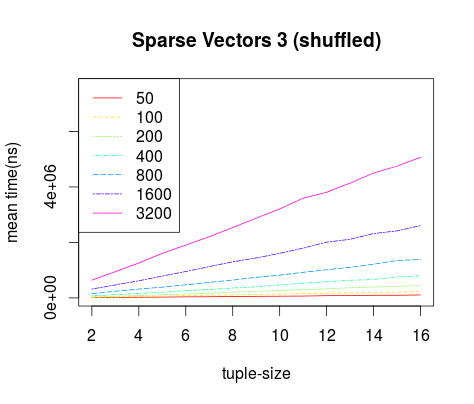
\includegraphics[width=0.35\textwidth]{gfx/times/shuffled/sparse_vectors_3.png}
                \label{fig:shuffled_sparse_vectors_3}
        }
    
        \caption[Effect of tuple size on the shuffled datasets for each of the evaluation techniques]{Effect of tuple size on the shuffled datasets for each of the evaluation techniques}\label{fig:sed_timings_techniques_shuffled}
\end{figure}

Figure \ref{fig:sed_timings_techniques_unshuffled} shows the growth of each mechanism on the unshuffled data.  The effect of early termination makes all levels of sparsity behave the same.  Whereas without early termination, the growth is larger for more sparse vectors.
\begin{figure}
        \centering
        \subfloat[Inverted Index]{
				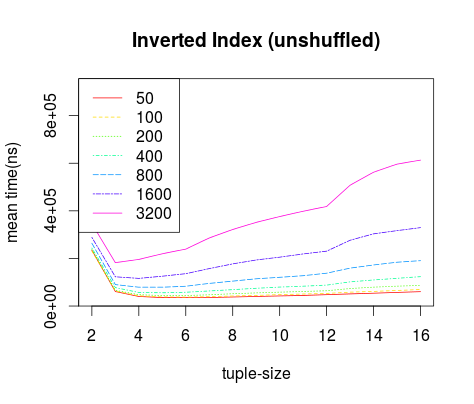
\includegraphics[width=0.35\textwidth]{gfx/times/unshuffled/inverted_index.png}
                \label{fig:unshuffled_inverted_index}
        }%
        ~ 
        \subfloat[Inverted Index ET]{
				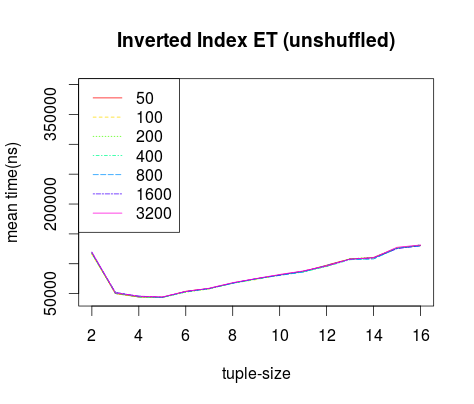
\includegraphics[width=0.35\textwidth]{gfx/times/unshuffled/inverted_index_et.png}
                \label{fig:unshuffled_inverted_index_et}
        }
        
         
        \subfloat[Sparse Vectors]{
				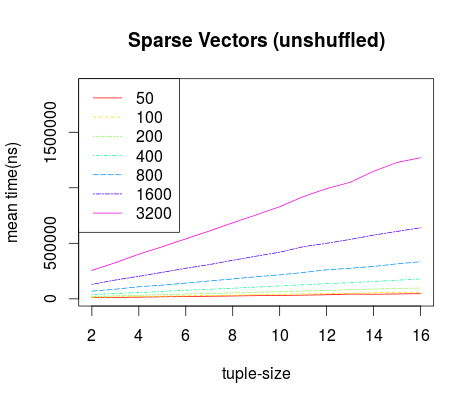
\includegraphics[width=0.35\textwidth]{gfx/times/unshuffled/sparse_vectors.png}
                \label{fig:unshuffled_sparse_vectors}
        }
        ~ 
        \subfloat[Sparse Vectors 2]{
				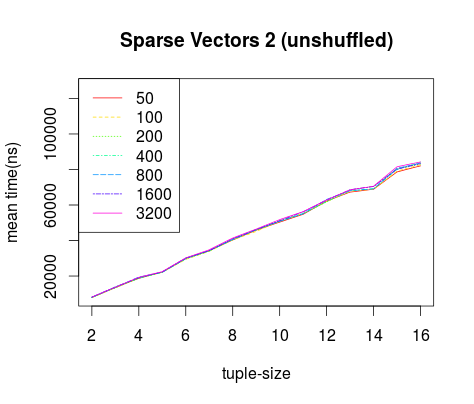
\includegraphics[width=0.35\textwidth]{gfx/times/unshuffled/sparse_vectors_2.png}
                \label{fig:unshuffled_sparse_vectors_2}
        }
        
        \subfloat[Sparse Vectors 3]{
				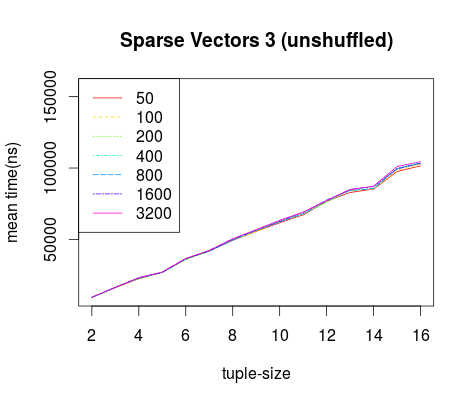
\includegraphics[width=0.35\textwidth]{gfx/times/unshuffled/sparse_vectors_3.png}
                \label{fig:unshuffled_sparse_vectors_3}
        }
    
        \caption[Effect of tuple size on the unshuffled datasets for each of the evaluation techniques]{Effect of tuple size on the unshuffled datasets for each of the evaluation techniques}\label{fig:sed_timings_techniques_unshuffled}
\end{figure}

% ------------------------------------------------------------------------------------------------------------------
Figure \ref{fig:sed_timings_dims_shuffled} compares the growth associated with increasing tuple size of each mechanism on the shuffled data.  On all levels of sparseness, using early termination increases the growth of cost associated with increasing the tuple size.
\begin{figure}
        \centering
        \subfloat[50 dims]{
				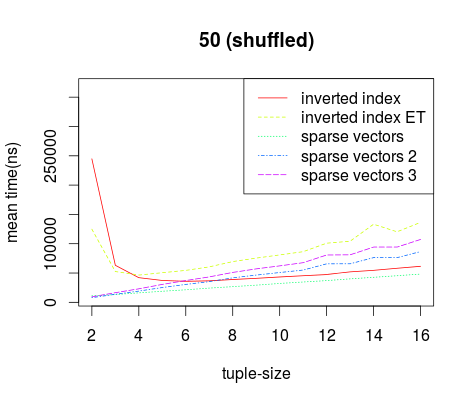
\includegraphics[width=0.35\textwidth]{gfx/times/shuffled/0050.png}
                \label{fig:shuffled_0050}
        }%
        ~ 
        \subfloat[100 dims]{
				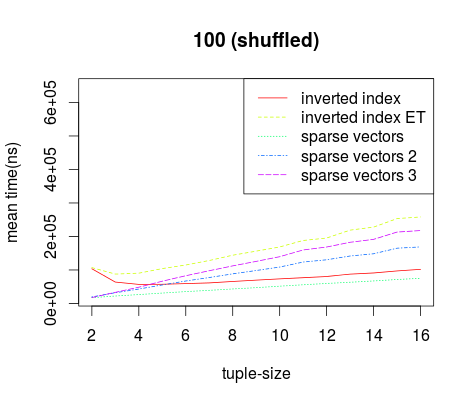
\includegraphics[width=0.35\textwidth]{gfx/times/shuffled/0100.png}
                \label{fig:shuffled_0100}
        }
        
         
        \subfloat[200 dims]{
				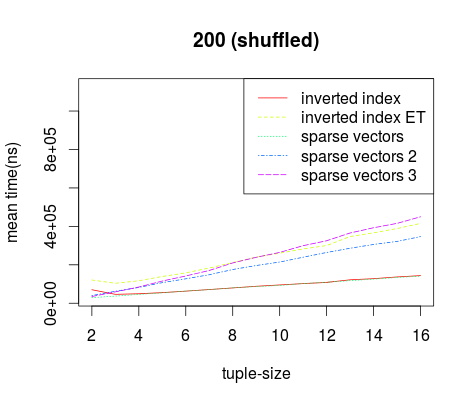
\includegraphics[width=0.35\textwidth]{gfx/times/shuffled/0200.png}
                \label{fig:shuffled_0200}
        }
        ~ 
        \subfloat[400 dims]{
				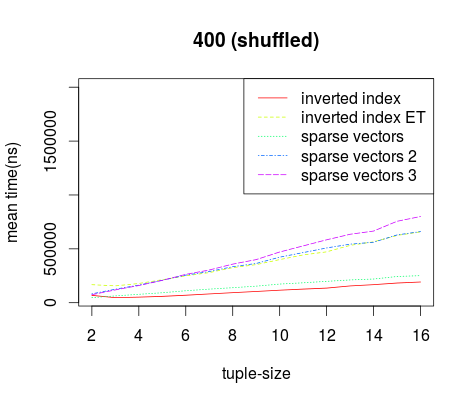
\includegraphics[width=0.35\textwidth]{gfx/times/shuffled/0400.png}
                \label{fig:shuffled_0400}
        }
        
        
        \subfloat[800 dims]{
				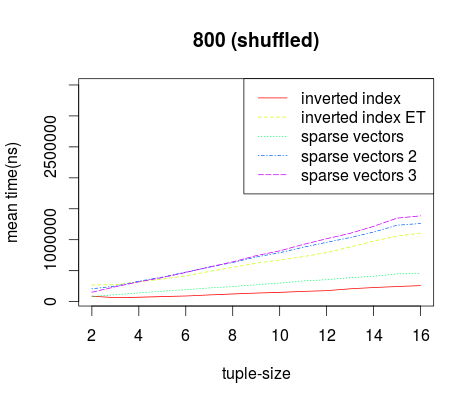
\includegraphics[width=0.35\textwidth]{gfx/times/shuffled/0800.png}
                \label{fig:shuffled_0800}
        }
         ~ 
        \subfloat[1600 dims]{
				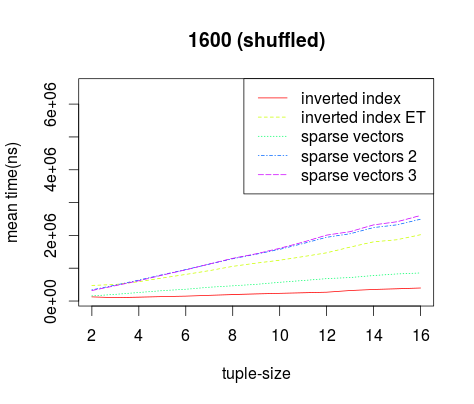
\includegraphics[width=0.35\textwidth]{gfx/times/shuffled/1600.png}
                \label{fig:shuffled_1600}
        }
        
        
        \subfloat[3200 dims]{
				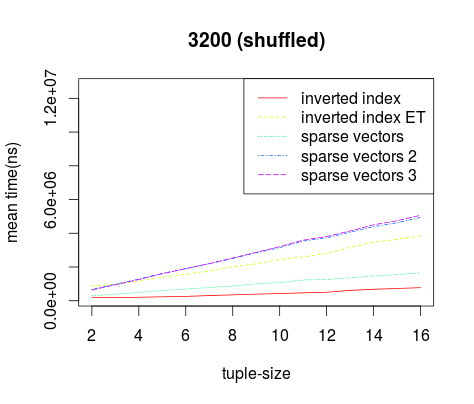
\includegraphics[width=0.35\textwidth]{gfx/times/shuffled/3200.png}
                \label{fig:shuffled_3200}
        }
    
        \caption[shuffled]{Shuffled}\label{fig:sed_timings_dims_shuffled}
\end{figure}

Figure \ref{fig:sed_timings_dims_unshuffled} compares the growth associated with increasing the tuple size of each mechanism on unshuffled data.  In this case we see that early termination has a positive effect.  Those with early termination grow more quickly.
\begin{figure}
        \centering
        \subfloat[50 dims]{
				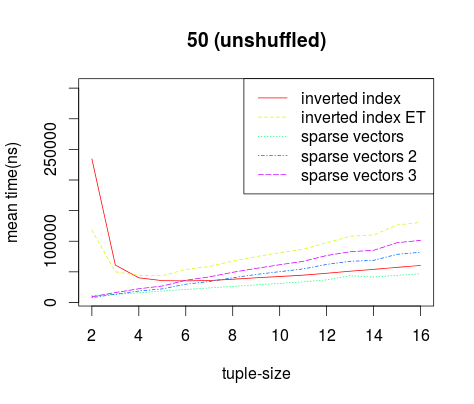
\includegraphics[width=0.35\textwidth]{gfx/times/unshuffled/0050.png}
                \label{fig:unshuffled_0050}
        }%
        ~ 
        \subfloat[100 dims]{
				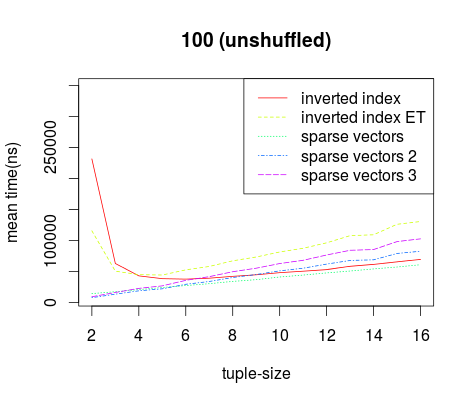
\includegraphics[width=0.35\textwidth]{gfx/times/unshuffled/0100.png}
                \label{fig:unshuffled_0100}
        }
        
         
        \subfloat[200 dims]{
				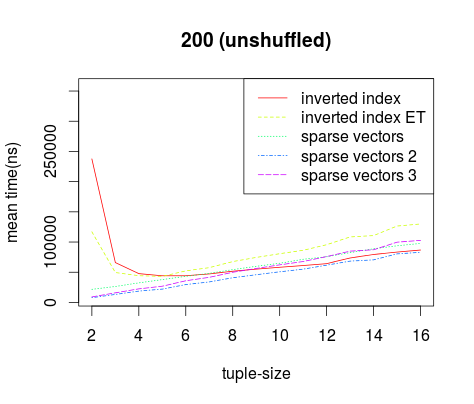
\includegraphics[width=0.35\textwidth]{gfx/times/unshuffled/0200.png}
                \label{fig:unshuffled_0200}
        }
        ~ 
        \subfloat[400 dims]{
				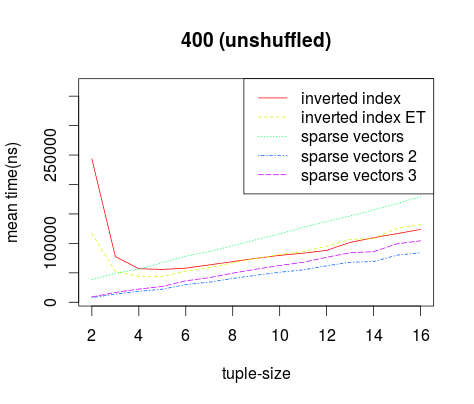
\includegraphics[width=0.35\textwidth]{gfx/times/unshuffled/0400.png}
                \label{fig:unshuffled_0400}
        }
        
        \subfloat[800 dims]{
				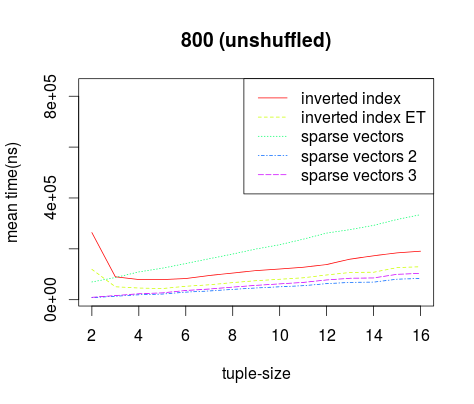
\includegraphics[width=0.35\textwidth]{gfx/times/unshuffled/0800.png}
                \label{fig:unshuffled_0800}
        }
        ~ 
        \subfloat[1600 dims]{
				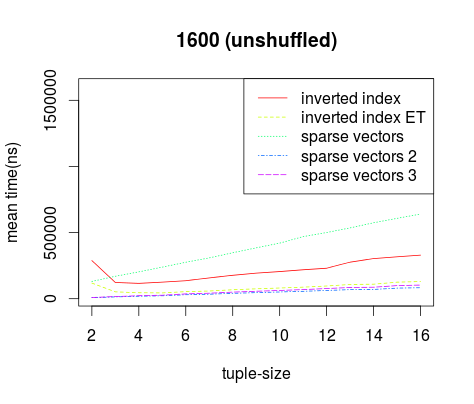
\includegraphics[width=0.35\textwidth]{gfx/times/unshuffled/1600.png}
                \label{fig:unshuffled_1600}
        }
        
        \subfloat[3200 dims]{
				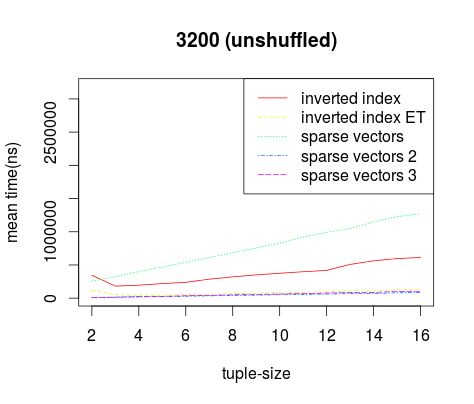
\includegraphics[width=0.35\textwidth]{gfx/times/unshuffled/3200.png}
                \label{fig:unshuffled_3200}
        }    
        \caption[Unshuffled]{Unshuffled}\label{fig:sed_timings_dims_unshuffled}
\end{figure}
%IDIM and threshold values may not be useful characteristics of the space. 
%With 95\% sparsity, the data is likely unevenly distributed in the space; threshold search values may not be significantly greater than those in the dense space. Real data sets bear out this intuition: similar objects are still similar in absolute terms independent of the dimensions for which they have no value.

%\begin{figure}[h]
%\centering
%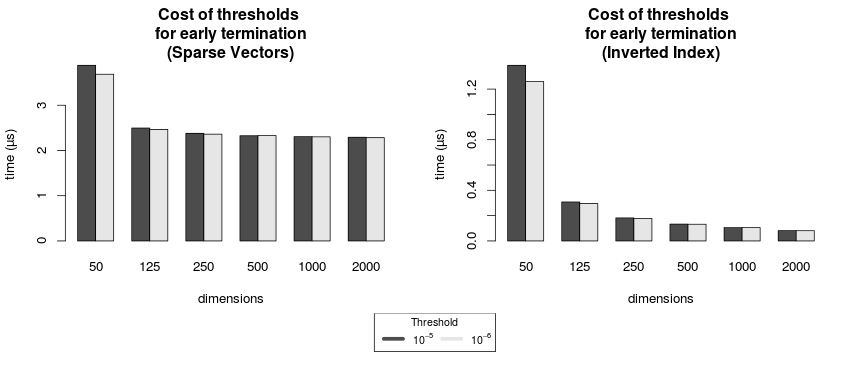
\includegraphics[width=0.9\columnwidth]{gfx/early_termination_thresholds}
%\caption[Early termination]{Cost of distance using early termination with thresholds $10^{-5}$ and $10^{-6}$}
%\label{fig:speedup_sed}
%\end{figure}

%For the dense benchmark set, definitions A, B and C gave almost the same times, which is unsurprising given there were no zero values. Exactly the same calculations took place in definitions A and B, while definition C produced a minor cost saving. This was further improved by the smaller threshold.  The saving by definition C was insignificant since the overhead of calculating the threshold values was almost as great.
%
%Definitions D and E gave a substantial saving, which is unexpected; definition D performed exactly the same set of calculations as definitions A and B. The only difference is the order in which the calculations were performed.  It may be the manner in which the data are fetched from slower to faster memory; inverted indices optimise this movement by moving the values in bigger chunks, allowing hardware optimisations to be used. While the movement here is between main and cache memory, the same principles apply with very large data sets between disk and main memory.
%
%Figure \ref{fig:speedup_sed} shows the threshold calculation of definition E was much more valuable in this context than its use in definition C. 
%While some of the calculation was amortised by the single traversal along the query vector; we do not fully understand the magnitude of the extra cost saving.
%
%%The trends as the overall dimensionality of the space increases fully vindicates our rationale. 
%As the overall dimensionality of the space was increased, definition A's times grew with the number of dimensions: first, the amount of data being moved through the processor memory increased; secondly, the rise in dimensions that have zero values in both operands yielded no extra saving.  As the size of the non-zero intersection diminished with increased sparsity, fewer calculations were performed by definition B, while the saving observed for definition C was lost; the cost of maintaining the threshold calculation outweighed the saving of early termination.  
%
%Although the same set of calculations were performed by definitions B and D, with definition D the volume of data passed though the processor cache decreased. The cost of maintaining the threshold calculation of Definition E, however, becomes proportionally greater, and since its advantage is increased with higher dimensionality, its relative advantage was lost.  It is still worth noting that, even at 2,000 dimensions, there was still a significant cost saving from this technique.
%
%Over the highest dimensions, a cost saving of almost two orders of magnitude was achieved, and the reasons for this should be maintained over very large data sets which are resident on disk rather than in memory.
\section{Conclusion}
The benefit associated with early termination and skipping dimensions clearly depends on the dataset being considered.  We examined the two extremes: when all the data have the same dimensions occupied and when they are populated randomly.  In the first instance, early termination clearly helped to reduce the cost of the calculation, but in the second the cost of maintaining the threshold calculation outweighed any saving.  In reality, most datasets will lie somewhere between these extremes, and may require some analysis to determine whether it would be appropriate to use these mechanisms.

